\begin{abstract}
Climate change and various anthropogenic factors significantly influence biodiversity and population evolutionary dynamics. To deepen our understanding of the mechanisms driving these disturbances within ecosystems, biologists employ phylogeographic approaches. These methods aim to establish the correlation between the genetic structure of populations and their geographical distribution, considering their current or historical geoclimatic history. 

We focus on developing bioinformatics \textbf{aPhyloGeo} tools to enhance phylogeographic analysis. Recognizing the urgency of the current climate crisis, we are conducting an in-depth analysis of the impact of extreme climatic parameters and environmental factors on Cumacea (crustaceans: Peracarida). Our approach includes a comparative study that validates our phylogeographic models against environmental data from the northern waters of the North Atlantic around Iceland. Concurrently, we are updating a Python package (\url{https://github.com/tahiri-lab/aPhyloGeo}), also available on \href{https://pypi.org/project/aphylogeo/}{PyPi}, to facilitate these complex analyses.
\end{abstract}

\section{Introduction}\label{introduction}
In the vast North Atlantic and subarctic region, the Icelandic area and its surrounding waters offer fascinating ecological interest \citep{schnurr_composition_2014, uhlir_adding_2021}. The waters surrounding Iceland contain a significant diversity of water bodies from various sources \citep{brix_iceage_2014}. These specific oceanographic and hydrographic characteristics shape benthic habitats through various parameters such as depth gradients, water mass indicators, and specific arrangement of habitats \citep{meisner_benthic_2014, uhlir_adding_2021}. Therefore, research in these areas enhances our understanding of deep-sea ecosystems and the patterns of biodiversity patterns found within them \citep{rogers2007corals, meisner_prefacebiodiversity_2018}.

Biological and environmental baseline data collected in these regions the IceAGE project, as well as its predecessors BIOFAR and BIOICE, which studied the biodiversity of the Faroe Islands and Iceland \citep{meisner_prefacebiodiversity_2018} are invaluable resources. They provide a crucial source of information for understanding two major issues facing present and future generations: the impact of climate change and mining on the seabed. The North Atlantic region around Iceland has been recognized for decades as a critical region for the regulation of global thermohaline \citep{meisner_prefacebiodiversity_2018}. The Greenland, Iceland and Norwegian (GIN) seas, as well as the high-latitude North Atlantic, play a crucial role in modern deep-sea ventilation. The surface waters of these regions are essential source regions for global deep-sea renewal, and are essentials for the circulation of thermohaline \citep{johannessen_relationship_1994}. One of the most important of these changes is the formation of cold, deep water \citep{meisner_prefacebiodiversity_2018}. With the loss of Arctic sea ice, the deep-sea formation process slowed down, likely impacting the flow dynamic and chemistry in the region studied during the IceAGE expedition \citep{meisner_prefacebiodiversity_2018}.

There is a growing international interest in deep-sea resource extraction \citep{mengerink_call_2014}. These operations target in particular mid-ocean ridges and other active geothermal areas. The ridges around Iceland include these types of areas, such as the Reykjanes Ridge, which is home to hydrothermal vent sites. Accurately and rigorously assessing the extent of damage and loss of ecosystem services caused by mining activities is difficult without robust baseline data \citep{meisner_prefacebiodiversity_2018}.

Crustaceans of the taxon Peracarida Calman, 1904, often constitute a significant portion of macrobenthic communities in Arctic and subarctic waters. They are widely dispersed across the continental shelf and slope of northern seas \citep{stransky_diversity_2010}. In this study, we focus on the peracarid taxon Cumacea Krøyer, 1846, which not only contribute to food webs, but are also essentials as indicators of marine habitat health \citep{stransky_diversity_2010}. The latter are mainly bottom-dwelling marine benthic crustaceans, spending a large part of their lives buried in or near sediments. Thus, Cumacea are presumed to have limited dispersal abilities and are unlikely to be able to move great distances \citep{uhlir_adding_2021}.

Unlike the benthic invertebrates that inhabit the rocky intertidal environments of the Northwest and Northeast Atlantic, the available information on the evolutionary history and dynamics of deep-sea benthic invertebrates in the North Atlantic remains limited \citep{jennings_phylogeographic_2014}. Although many studies reveal interesting patterns of genetic distribution of benthic invertebrates from the deep sea (e.g. \citep{wilson_historical_1998, havermans_genetic_2013}). However, it is fundamental to better understand the origin and demography of deep Atlantic biota in order to grasp its relationship with ongoing climate change which should be considered a factor in range expansion of deep-sea fauna \citep{jennings_phylogeographic_2014}.

In the context of the current climate emergency, this study aims to undertake an in-depth analysis of the influence of extreme climatic parameters and environmental peculiarities on Cumacea (crustaceans: Peracarida). Specifically, we wish to determine whether there is a correlation between the genetic information of regions of the mitochondrial 16S rRNA gene of Cumacea species sampled and the physical characteristics of their habitats. Our approach includes a comparative study to validate different phylogeographic models by comparing them with environmental factors found in the waters of the North Atlantic seas around Iceland. Additionally, we will update a Python package (in beta) to facilitate these complex analyses.

\section{Related Works}\label{related-works}
Many studies have investigated the relationship between genetics and the climatic conditions of their study region, showing how organisms acclimatize to their environnement over time. These studies have provided a better understanding of how organisms adapt to their habitat and evolve in it over time \citep{fc_genomic_2012}. They have also helped develop conservation plans to maintain biodiversity and protect endangered species by designing how populations are adapted to their environment \citep{balkenhol_identifying_2009}.

\cite{koshkarov_phylogeography_2022} proposed a phylogeographic approach based on an algorithm called aPhyloGeo to study the correlation between Severe acute respiratory syndrome coronavirus 2 (SARS-CoV-2) variants and their geographical characteristics. More recently, \cite{li_aphylogeo-covid_2023} have developed an interactive platform called aPhyloGeo-Covid to facilitate these analyses.  We elaborate on the aPhyloGeo software as well as its use in this study later in this article.

The correlation between genetics and environmental parameters has been confirmed in studies of a variety of organisms, supporting the influence of habitat characteristics on genetic diversity \citep{colosimo_widespread_2005, cheviron_genomic_2012}. A study by \cite{ghalambor_adaptive_2007} has demonstrated that habitat characteristics, such as water temperature, can affect the genetics of guppy populations (\emph{Poecilla reticulata}) by shaping their phenotypic plasticity as well as by promoting rapid genetic adaptation. \cite{cheviron_genomic_2012} also concluded that there was a correlation between vertebrate genetics and habitat properties, particularly in extreme environments such as high altitudes. This correlation between genetics and environmental characteristics was also supported by the results of studies of Threespine Sticklebacks \citep{colosimo_widespread_2005}. Those results are to be expected considering that species acclimatization to climate change is often the result of the interaction between genetic variation among populations and selection pressures caused by environmental changes \citep{hoffmann_climate_2011}.

However, studies have highlighted the complexity of the relationships between genetics and the environment that can be influenced by many factors such as genotype-environment interaction and natural selection. This can make it difficult to identify unambiguous causal relationships between these two parameters \citep{balkenhol_identifying_2009}. Other studies mention that it is difficult to distinguish between the direct and indirect effects of the environment on genetics \citep{manel_perspectives_2010, balkenhol_landscape_2019}. Studies of the effect of the environment on the genetics of organisms may be limited by the methods available to measure genetic and environmental characteristics, as well as by logistical constraints related to data collection and generation \citep{manel_perspectives_2010, shafer_widespread_2013}. To our knowledge, this last point must contribute in particular to the fact that research on the environment and genetics of Cumacea is little explored, but they remain importants for understanding how these organisms adapt to fluctuating environmental conditions. 

As stipulated in hypothesis of Darwin, individuals best adapted to their environment are likely to survive, reproduce and evolve. The objective of this study is to deepen and strengthen the natural selection hypothesis by examining whether there are one or more locations within DNA sequence of Cumacea of the mitochondrial 16S rRNA gene that could correlate not only the portions of the sequence (windows), but the Cumacea to their environment.

\section{Materials and Methods}\label{materials-methods}

\subsection{Description of the data}
The study area is located in a northern area of the North Atlantic, including the Icelandic Sea, the Denmark Strait, and the Norwegian Sea. The specimens included in this study were collected during the IceAGE project (Icelandic marine Animals: Genetic and Ecology; Cruise ship M85/3 in 2011; \citep{brix_iceage_2014}) that explored the deep continental slopes and abyssal waters around Iceland \citep{meisner_prefacebiodiversity_2018}. The sampling period for the specimens included in this study is from August 30 to September 22, 2011, and they were collected in a depth range of 316-2568 m. A description of the sampling plan, sample processing, the steps of DNA extraction, PCR amplification and sequencing, as well as the extracted and aligned DNA sequences, are available in the article by \citep{uhlir_adding_2021}.

\subsection{Data pre-processing}
We considered data from the IceAGE project as well as the derived data from the BOLD Systems database, both of which are available via the article by \citep{uhlir_adding_2021}. Given the large scope of attributes from these databases, we made a succinct selection of the number of attributes and samples across them. Thus, we omitted attributes that were not relevant to the context of this study, that were completely or nearly invariable (non-numerical data) as well as those that had abundant missing data (> 95\%). We considered 62 specimens of the dataset available (495) from the IceAGE project.

Subsequently, we calculated the variance for each of the selected numeric attributes in order to eliminate those with zero or low variance (cut-off ≥ 0.1):

\begin{equation}
S^2 = \frac{\sum_{i=1}^{n} (x_i - \bar{x})^2}{n-1}
\end{equation}

where \( S^2 \) is the variance of the sample, \( x_i \) represents each value in the dataset, \( \bar{x} \) the average of all values in the dataset, and \( n \) the number of values in the dataset.

Of the previously selected numerical attributes, only salinity was removed (\( S^2 = 0.02146629 \)). This selection of attributes and data resulted in a data table containing 62 rows (\( n=62 \)) and 18 columns (number of attributes). 

From the IceAGE database, 14 attributes were selected. These consist of the geographical coordinates such as longitude (decimal) and latitude (decimal) taken at the beginning (see Figure \ref{fig:fig1}a and \ref{fig:fig1}b) and at the end of sampling. The increase in latitude, in particular, has been highlighted by several studies as being linked to the decline of marine biodiversity on a global scale \citep{lambshead_latitudinal_2000, gage_diversity_2004}. These geographic data are divided into five sectors across the seas around Iceland: the Denmark Strait (\( n=28 \)), the Iceland Basin (\( n=15 \)), the Irminger Basin (\( n=12 \)), the Norwegian Sea (\( n=4 \)) and the Norwegian Basin (\( n=3 \)). For the environmental attributes in this database, we included the depth (m) at the beginning (see Figure \ref{fig:fig1}c) and end of sampling as well as the temperature (\( \degree C \)) (see Figure \ref{fig:fig1}d) and oxygen concentration (mg/L) (see Figure \ref{fig:fig1}e) of the water depending on the depth at which the specimens were sampled. These properties of water bodies are drivers of deep-sea biodiversity and biogeography with oxygen being a limiting factor for living organisms \citep{keeling_ocean_2010}. In addition to these contributions, the increase in depth \citep{rex_global_2006, costello_marine_2017} as well as the decrease in water temperature at depth \citep{lambshead_latitudinal_2000} are also factors in the loss of marine biodiversity on a global scale. Meteorological parameters such as wind speed (m/s) (see Figure \ref{fig:fig1}f) and wind direction at the beginning and end of sampling were also included in our data given the contribution of wind to the restructuring of the benthic ecosystem through water transport \citep{waga_recent_2020, saeedi_environmental_2022}. The wind direction at the start of sampling consists of six orientations: South-West (\( n=22 \)), South (\( n=15 \)), North-East (\( n=9 \)), South-South-East (\( n=9 \)), North-West (\( n=5 \)) and East (\( n=2 \)); while the one at the end of sampling is made up of seven orientations: South (\( n=15 \)), South-West (\( n=15 \)), North-East (\( n=9 \)), West-South-West (\( n=7 \)), South-East (\( n=6 \)), North-North-West (\( n=5 \)), South-South-East (\( n=3 \)) and East (\( n=2 \)). In addition, we have included the sedimentary characteristics of the sampling sites as factors influencing the distribution of Cumacea \citep{uhlir_adding_2021} and which, for the purposes of this study, fall into six categories: mud (\( n=30 \)), sandy mud (\( n=15 \)), sand (\( n=9 \)), forams (\( n=3 \)), muddy sand (\( n=3 \)) and gravel (\( n=2 \)).

In the BOLD Systems database, taxonomic ranks such as family, genus, and species of the sampled Cumacea were included in our data. These are composed of seven families of Cumacea: Diastylidae (\( n=21 \)), Lampropidae (\( n=13 \)), Leuconidae (\( n=12 \)), Nannastacidae (\( n=7 \)), Bodotriidae (\( n=4 \)), Ceratocumatidae (\( n=3 \)) and Pseudocumatidae (\( n=2 \)). A total of 21 species of Cumacea are found in our sample (see Figure \ref{fig:fig2}).

The habitat and water mass of the sampling points are the only attributes that were taken directly via Table 1 of \citep{uhlir_adding_2021}. Thus, the definitions of water bodies described by \citep{hansen_north_2000, brix2010distribution, ostmann_marine_2014} were used as a reference for the GIN seas around Iceland: Arctic Polar Water (APW, \( n=15 \)), Iceland Sea Overflow Water (ISOW, \( n=15 \)), North Atlantic Water (NAW, \( n=9 \)), Arctic Polar Water/Norwegian Sea Arctic Intermediate Water (APW/NSAIW, \( n=7 \)), warm Norwegian Sea Deep Water (NSDWw, \( n=8 \)), Labrador Sea Water (LSW, \( n=3 \)), cold Norwegian Sea Deep Water (NSDWc, \( n=3 \)) and Norwegian Sea Arctic Intermediate Water (NSAIW, \( n=2 \)) (see Figure \ref{fig:fig3}). In terms of habitat, we considered the three categories used in \citep{uhlir_adding_2021}: deep sea (\( n=38 \)), shelf (\( n=15 \)) and slope (\( n=9 \)) (see Figure \ref{fig:fig4}).

In order to better interpret the relation and evolutionary responses of benthic species, genetic data are needed \citep{wilson_speciation_1987, uhlir_adding_2021}. The aligned DNA sequence of the mitochondrial 16S rRNA gene region of each of the samples will be included in our analyses. In order to understand  Thus, we consider 62 of the 306 aligned DNA sequences that were used for phylogenetic analyses of \citep{uhlir_adding_2021}. Since some of the specimens in our sample have their DNA sequence aligned duplicated, or even quadrupled with a difference of one to two nucleotides, we considered the longest aligned DNA sequence for each specimen. Figures  \ref{fig:fig1},  \ref{fig:fig2}, \ref{fig:fig5} and \ref{fig:fig6} were made from Python 3.11, while Figures \ref{fig:fig3} and \ref{fig:fig4} were made from RStudio Desktop 4.3.2.

\subsection{aPhyloGeo software}

For our analyses, we use the cross-platform Python software aPhyloGeo designed to analyze phylogenetic trees using climate parameters. Developed by Nadia Tahiri, Georges Marceau and David Beauchemin, the latter offers tools to study the correlations between the genetics of species and their habitats, thus allowing the understanding of the evolution of species under different environmental conditions. The software process takes place in three main steps. 

    The first step is to collect Cumacea DNA sequences of sufficient quality for the requirements of our results \citep{koshkarov_phylogeography_2022}. A total of 62 Cumacea samples were selected to represent 62 sequences of the gene mitochondrial 16S rRNA. Subsequently, we included 6 climatic factors, namely the temperature and O2 concentration of the water as well as the wind speed at the beginning and end of the sampling. We also included 6 geographical factors, such as the latitude, longitude and depth of sample collection at the beginning and end of sampling were also considered among our geographical parameters.

    In the second step, the trees were generated with climatic, geographical and genetic data. For the geographic parameters, we calculated the dissimilarity between each pair of data from different geographic conditions, which produced a symmetric square matrix. From this matrix, the neighbor junction algorithm was used to design the climate tree. The same approach was applied to climatic and genetic data. Using the 62 sequences of the gene of mitochondrial 16S rRNA, phylogenetic reconstruction is repeated to build gene trees, considering only the data within a range that moves along the alignment. This displacement can vary depending on the steps and window size set by the user (their length is defined by the number of base pairs (pb)) \citep{koshkarov_phylogeography_2022}.

    In the third step, the phylogenetic trees built in each sliding window are compared to climatic and geographic parameters using the Robinson-Foulds (RF) Distance \citep{robinson_comparison_1981, koshkarov_phylogeography_2022}, the Normalized Robinson-Foulds Distance, the Euclidean Distance and the Least-Squares Distance. The distance was normalized by $2n-6$, where $n$ represents the number of taxa. The approach also considers bootstraping. Thus, the use of the sliding window ensures detailed identification of regions with high genetic mutation rates \citep{koshkarov_phylogeography_2022}.

In short, we want to demonstrate a potential correlation between parts of the genes containing a high rate of mutations according to the geographical distribution of Cumacea samples (see \autoref{lst:main}).

%\autoref{lst:main}.
\begin{lstlisting}[label=lst:main,language=Python,caption=aPhyloGeo’s main function]
    if __name__ == "__main__":
        print(titleCard + "\n")

        # load params 
        Params.load_from_file()
        sequenceFile = utils.loadSequenceFile(Params.reference_gene_filepath)
        align_sequence = AlignSequences(sequenceFile)

        climatic_data = pd.read_csv(Params.file_name)

        print("\nStarting alignement")
        start_time = time.time()
        alignements = align_sequence.align()

        geneticTrees = utils.geneticPipeline(alignements.msa)
        trees = GeneticTrees(trees_dict=geneticTrees, format="newick")
        end_time = time.time()
        elapsed_time = round(end_time - start_time, 3)
        print(f"Elapsed time: {elapsed_time} seconds")

        climaticTrees = utils.climaticPipeline(climatic_data)
        utils.filterResults(climaticTrees, geneticTrees, climatic_data)

        alignements.save_to_json(f"./results/aligned_{Params.reference_gene_file}.json")
        trees.save_trees_to_json("./results/geneticTrees.json")
\end{lstlisting}

\section{Metrics}\label{metrics}
The following section present a more concise versions of the formulas mentioned in the third step of the previous section :

\subsection{Robinson-Foulds Distance (RF Distance)}\label{RF}
The Robinson-Foulds distance measures the dissimilarity between two phylogenetic trees. It counts the number of splits (bipartitions) that are present in one tree but not the other (see \autoref{lst:robinsonFoulds}).

\[ \text{RF}(T_1, T_2) = | \Sigma(T_1) \Delta \Sigma(T_2) | \]

where \( \Sigma(T_1) \) and \( \Sigma(T_2) \) are the sets of splits in trees \( T_1 \) and \( T_2 \).

%\autoref{lst:robinsonFoulds}.
\begin{lstlisting}[label=lst:robinsonFoulds,language=Python,caption=Python script for calculating the Robinson-Foulds distance using the ete3 package in aPhyloGeo package]
    def robinsonFoulds(tree1, tree2):
        rf = 0
        tree1_newick = ete3.Tree(tree1.format("newick"), format=1)
        tree2_newick = ete3.Tree(tree2.format("newick"), format=1)

        rf, rf_max, common_leaves, x2, x3, x4, x5 = tree1_newick.robinson_foulds(tree2_newick, unrooted_trees=True)
        if len(common_leaves) == 0:
            rf = 0

        return rf, rf / rf_max
\end{lstlisting}


\subsection{Normalized Robinson-Foulds Distance}\label{RFnorm}
The normalized Robinson-Foulds distance scales the RF distance to account for the size of the trees, giving a value between 0 and 1.

\[ \text{RF}_{\text{norm}}(T_1, T_2) = \frac{| \Sigma(T_1) \Delta \Sigma(T_2) |}{| \Sigma(T_1) | + | \Sigma(T_2) |} \]

\subsection{Euclidean Distance}\label{euclidean}
The Euclidean distance between two points in a multi-dimensional space is the length of the line segment connecting them (see \autoref{lst:euclideanDist}).

For points \( \mathbf{p} = (p_1, \ldots, p_n) \) and \( \mathbf{q} = (q_1, \ldots, q_n) \):

\[ d_{\text{Euclidean}}(\mathbf{p}, \mathbf{q}) = \sqrt{\sum_{i=1}^{n} (p_i - q_i)^2} \]

%\autoref{lst:euclideanDist}.
\begin{lstlisting}[label=lst:euclideanDist,language=Python,caption=Python script for calculating the Euclidean distance distance using the ete3 package in aPhyloGeo package]
    def euclideanDist(tree1, tree2):
        ed = 0
        tns = dendropy.TaxonNamespace()
        tree1_tc = dendropy.Tree.get(data=tree1.format("newick"), schema="newick", taxon_namespace=tns)
        tree2_tc = dendropy.Tree.get(data=tree2.format("newick"), schema="newick", taxon_namespace=tns)
        tree1_tc.encode_bipartitions()
        tree2_tc.encode_bipartitions()
        ed = dendropy.calculate.treecompare.euclidean_distance(tree1_tc, tree2_tc)

        return ed
\end{lstlisting}

\subsection{Least-Squares Distance}\label{LS}
The Least-Squares distance measures the discrepancy between observed and estimated values, often used in regression analysis (see \autoref{lst:LeastSquare}).

For observed values \( y_i \) and estimated values \( \hat{y}_i \):

\[ d_{\text{LS}} = \sum_{i=1}^{n} (y_i - \hat{y}_i)^2 \]

These formulas succinctly describe the methods used to measure distances and dissimilarities in various contexts.

%\autoref{lst:LeastSquare}.
\begin{lstlisting}[label=lst:LeastSquare,language=Python,caption=Python script for calculating the Least-Square distance using the ete3 package in aPhyloGeo package]
    def leastSquare(tree1, tree2):
        ls = 0.00
        leaves = tree1.get_terminals()

        leavesName = list(map(lambda x: x.name, leaves))
        for i in leavesName:
            leavesName.pop(0)
            for j in leavesName:
                d1 = tree1.distance(tree1.find_any(i), tree1.find_any(j))
                d2 = tree2.distance(tree2.find_any(i), tree2.find_any(j))
                ls += abs(d1 - d2)
        return ls
\end{lstlisting}

\section{Results}\label{results}

Figure \ref{fig:fig1} shows the extent and variability of the dataset for three geographic attributes, namely latitude (decimal) and longitude (decimal) at the start of sampling and depth (m) at specimen collection, as well as three environmental attributes, such as wind speed at the start of sampling (m/s) and temperature (\( \degree C \))) and the oxygen concentration of the water (mg/L) based on the depth at which the samples were collected.

\begin{figure}[]
    \centering
    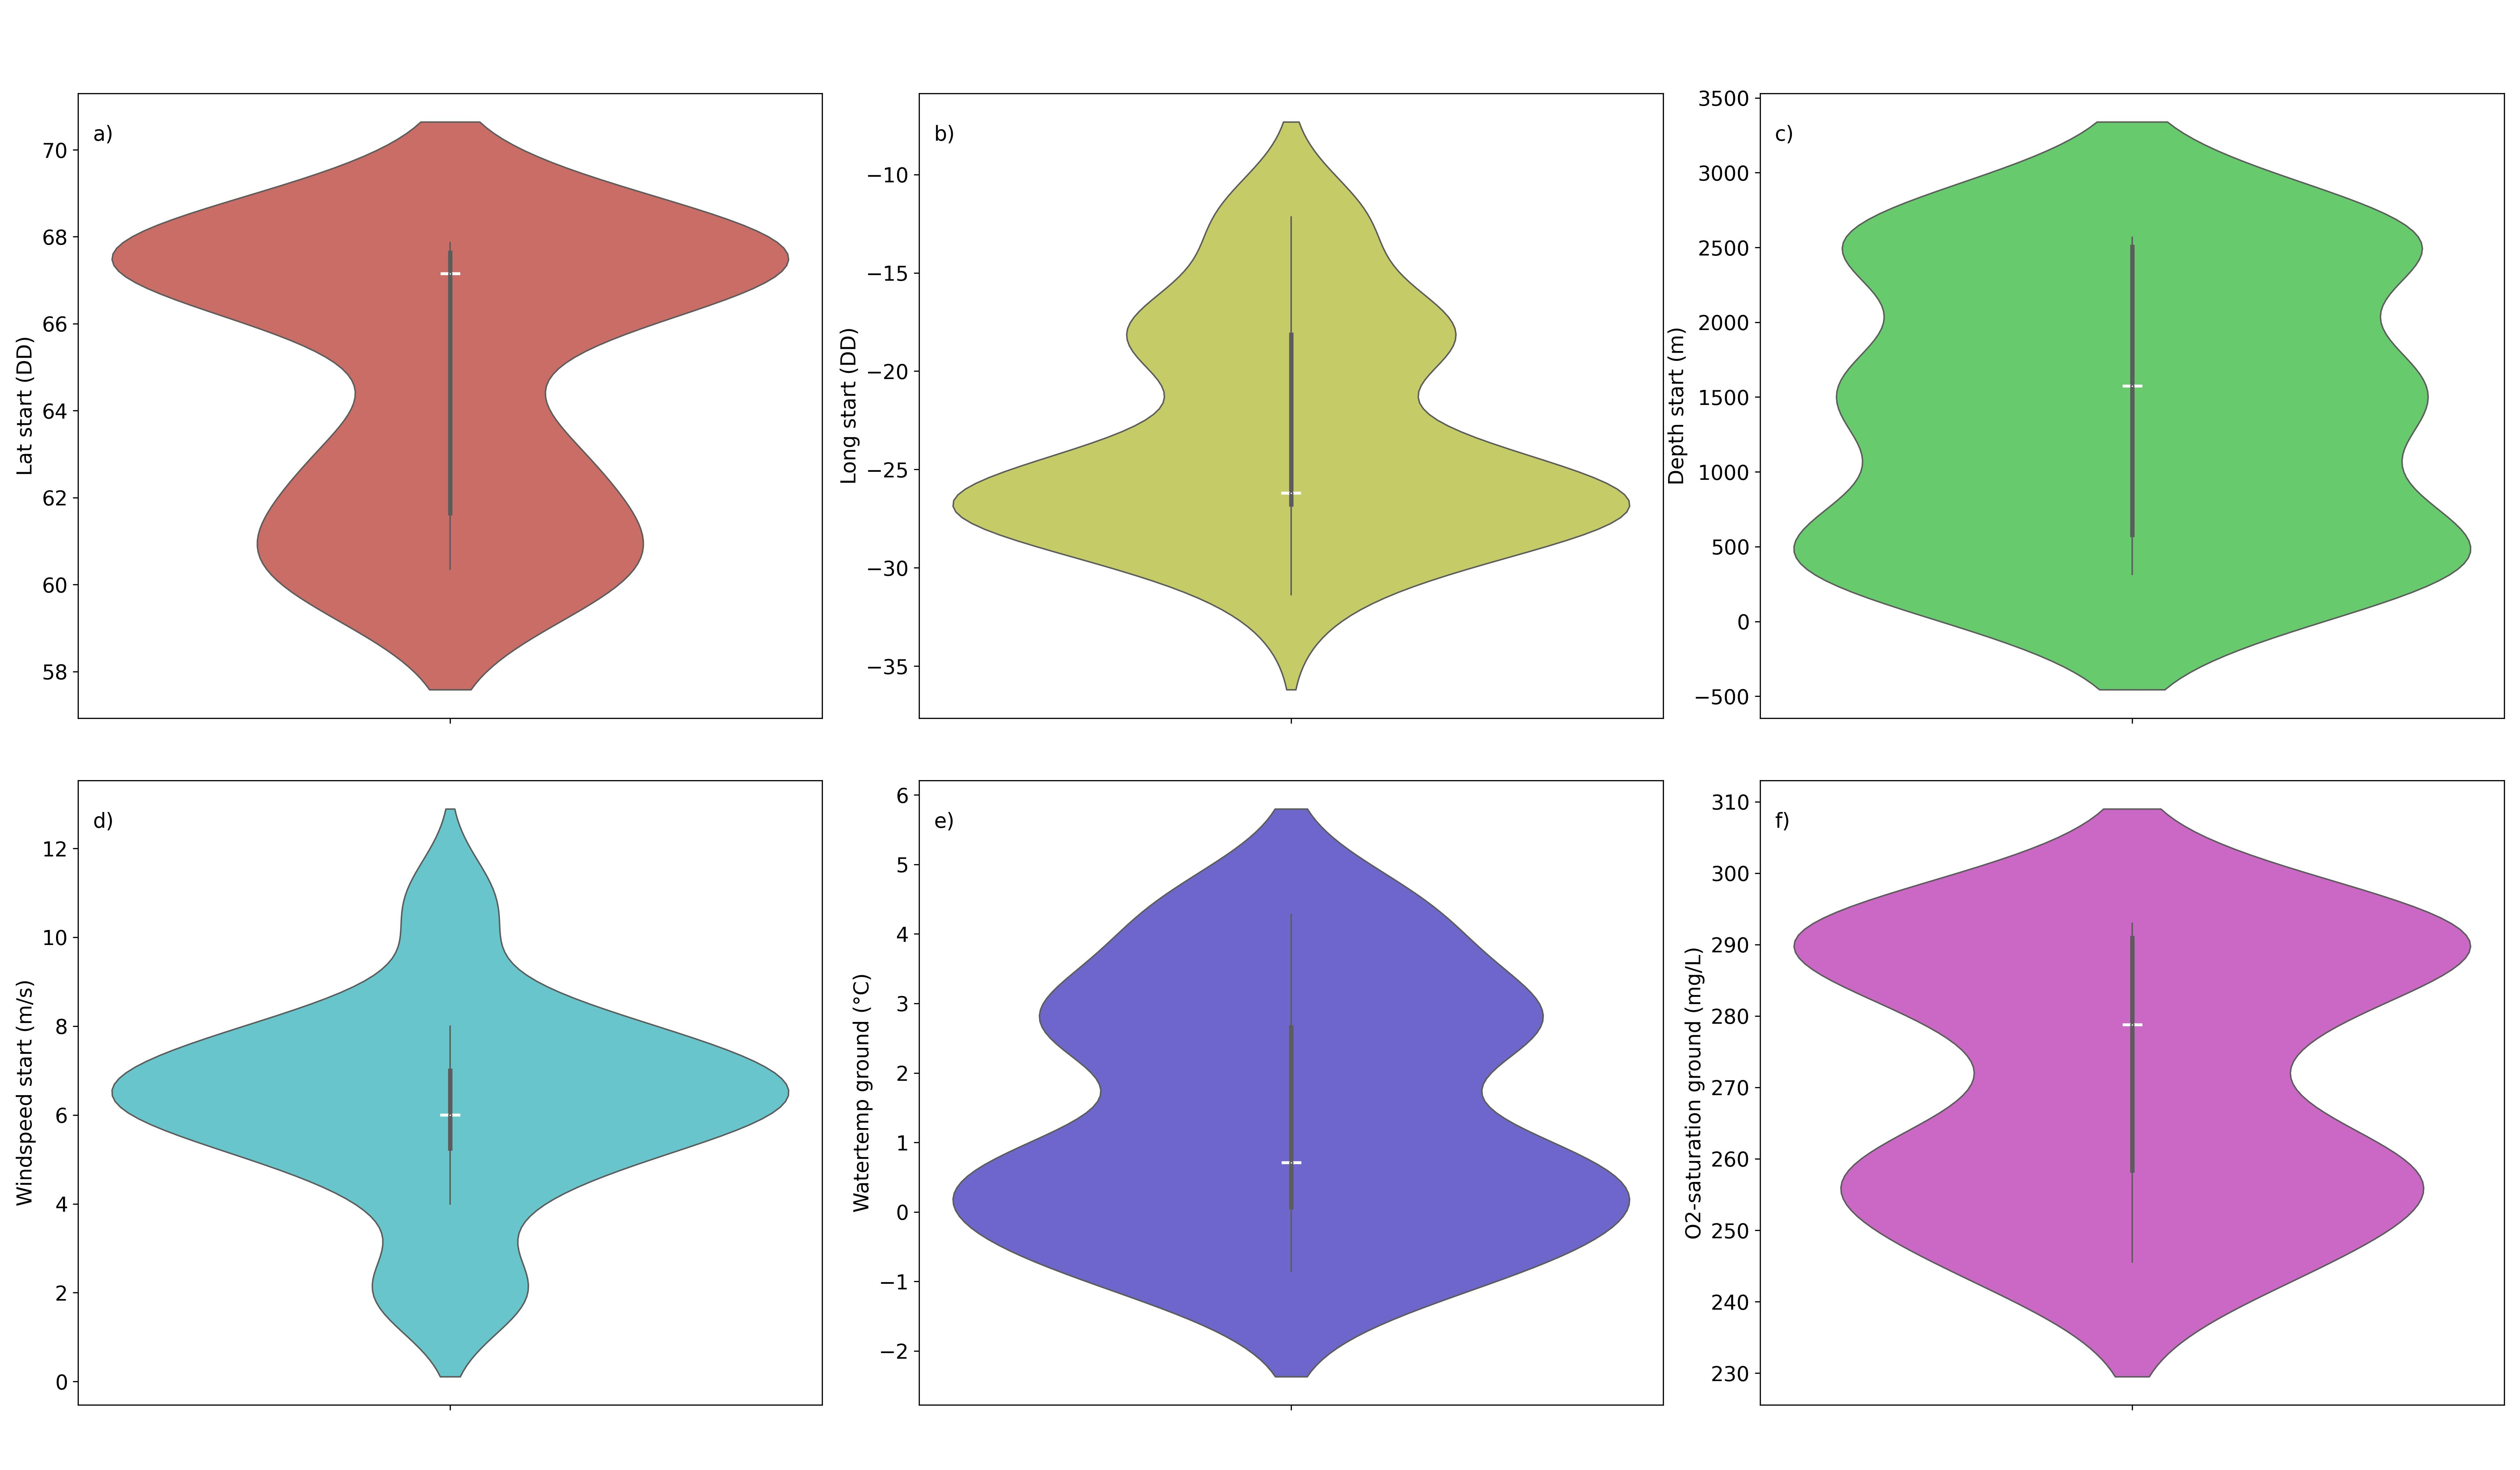
\includegraphics[width=0.7\textwidth]{figure1.jpg}
    \caption{Violin diagrams of six geographical and environmental attributes in our sample. a) Latitude (decimal) at the beginning of sampling (red); b) Longitude (decimal) at the beginning of sampling (yellow); c) Depth (m) at the start of sampling (green); d) Wind speed (m/s) at the beginning of sampling (light blue); e) Water temperature (°C) according to the depth at which the specimens were collected (dark blue); (f) Oxygen concentration (mg/L) according to the depth at which the specimens were sampled (pink). The mean, median, standard deviation (Std, Dev), 1st quartile (Q1), and 3rd quartile (Q3) of the dataset for each attribute are shown in the top right corner of each chart. \label{fig:fig1}}
\end{figure}

These digraphs are critical to designing the conditions of the habitats where the samples were collected, as high variability in the data may indicate heterogeneous habitats, while low variability dictates more homogeneous habitats. These diagrams can provide visual evidence that can support or refute our hypothesis regarding the relationship between these environmental variables and Cumacea genetics. For example, if a correlation is found between temperature and certain genetic variations, this may support that temperature influences the genetic structure of Cumacea populations. Thus, these violin graphs allow us to highlight rare environmental events or unique habitats that can have a significant impact on Cumacea genetics. 

The mean, median, standard deviation, and 1st and 3rd quartiles are represented in the top right corner of each of the six charts. These make it possible to identify general trends in the data as well as irregularities or extreme values in our data. For example, a large dissimilarity between the mean and the median may indicate the presence of extreme values, as is the case for depth (m) at the beginning of sampling. Large variations in standard deviation may indicate that some environmental variables are more variable and could have a different impact on Cumacea genetics, as is also the case for depth at the beginning of sampling. 

The latitude curve at the beginning of sampling has a bimodal asymmetric shape. The longitude distribution shows two peaks, suggesting that the samples stem from two dominant latitudinal regions at the beginning of sampling. This bimodality could potentially refer to a geographical separation of samples into two different groups. This type of curve is also present for the longitude at the beginning of the sampling as well as for the temperature and oxygen concentration of the water where the samples were collected. The wind speed at the beginning of sample collection has a symmetrical shape, similar to a normal one, with a high concentration of data around the median (6.00 m/s). This indicates that wind conditions at the beginning of sampling must have been relatively stable. The depth curve at the beginning of sample collection has a multimodal shape with three main peaks. This suggests that the samples were collected at various distinct depths, reflecting the diversity of benthic habitats.

\begin{figure}[]
    \centering
    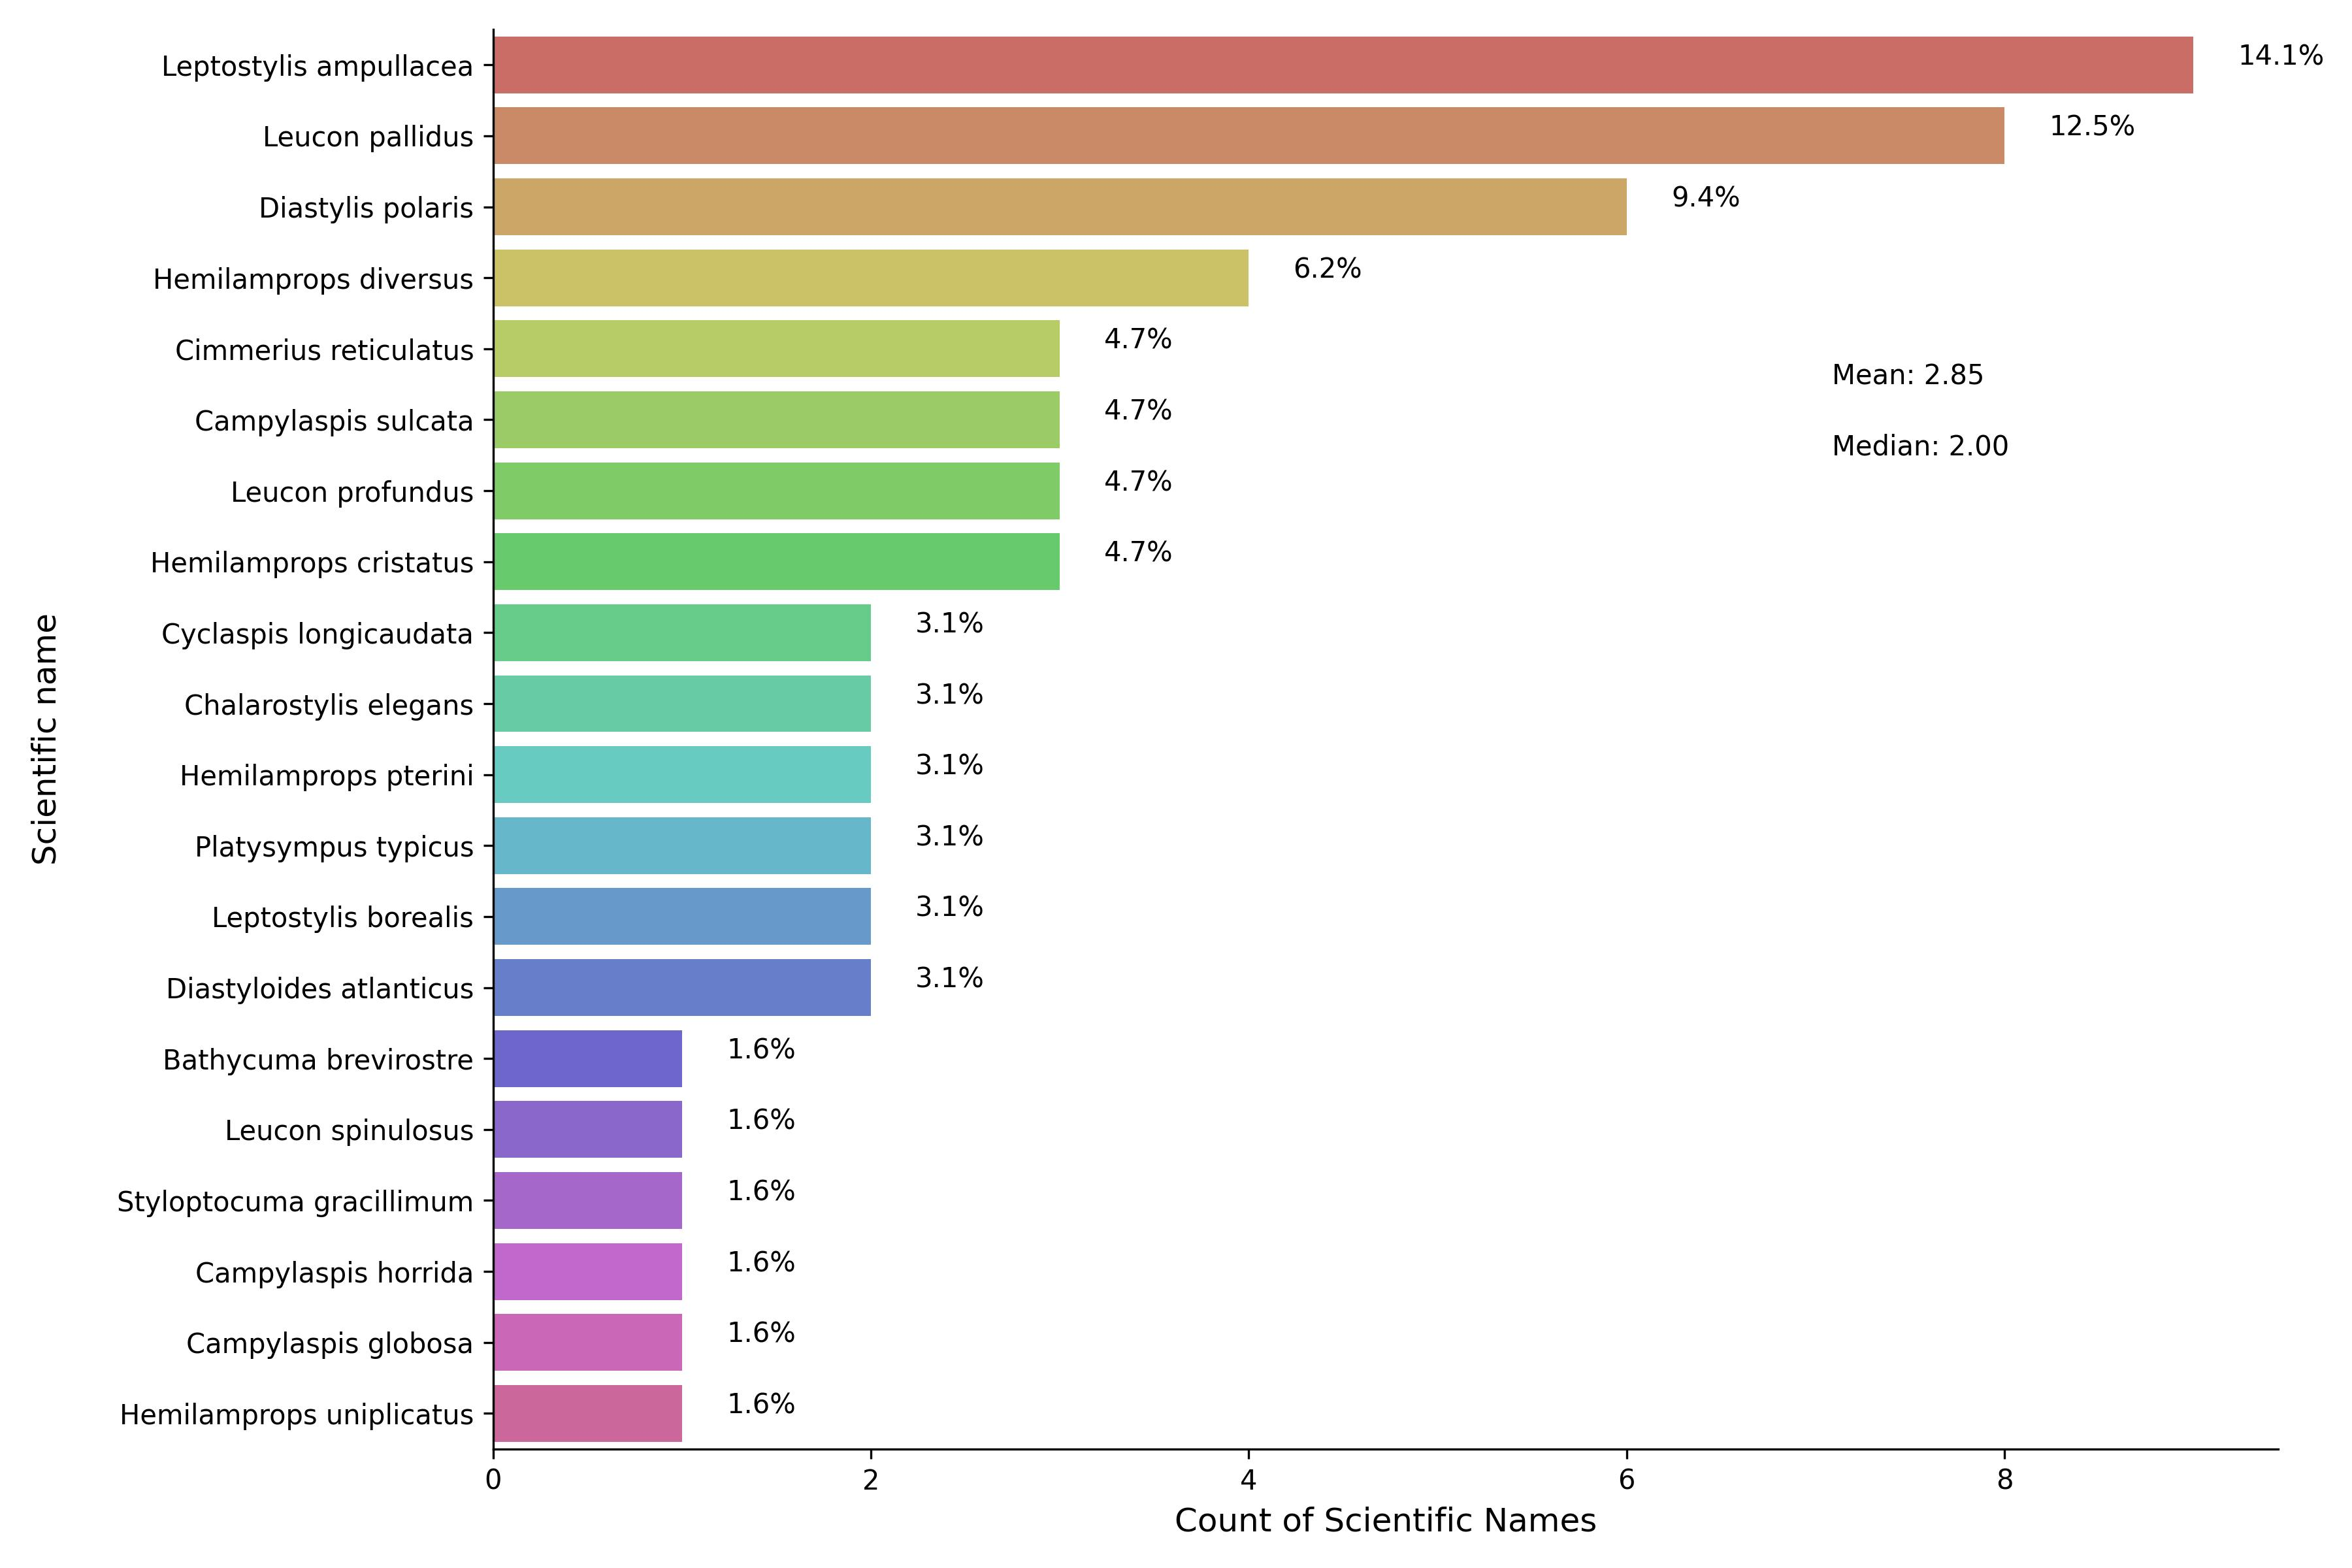
\includegraphics[width=0.7\textwidth]{figure2.jpg}
    \caption{Histogram of the frequencies of Cumacea species found in our sample. The percentages above the frequency bands represent the relative percentage of each species in the sample. The mean and median of the distribution are shown in the right corner of the histogram. \label{fig:fig2}}
\end{figure}

Figure \ref{fig:fig2} presents the distribution and diversity of the different Cumacea species found in our sample and our analyses in order to visualize the most represented species (Leptostylis ampullacea and Leucon pallidus) and those that are less represented (Bathycuma brevirostre, Leucon spinulosus, Styloptocuma gracillimum, Campylaspis horrida, Campylaspis globosa and Hemilamprops uniplicatus). This figure can potentially help us identify which species have genetic diversity related to their geographical distribution as well as to one or more local adaptations.

\begin{figure}[]
    \centering
    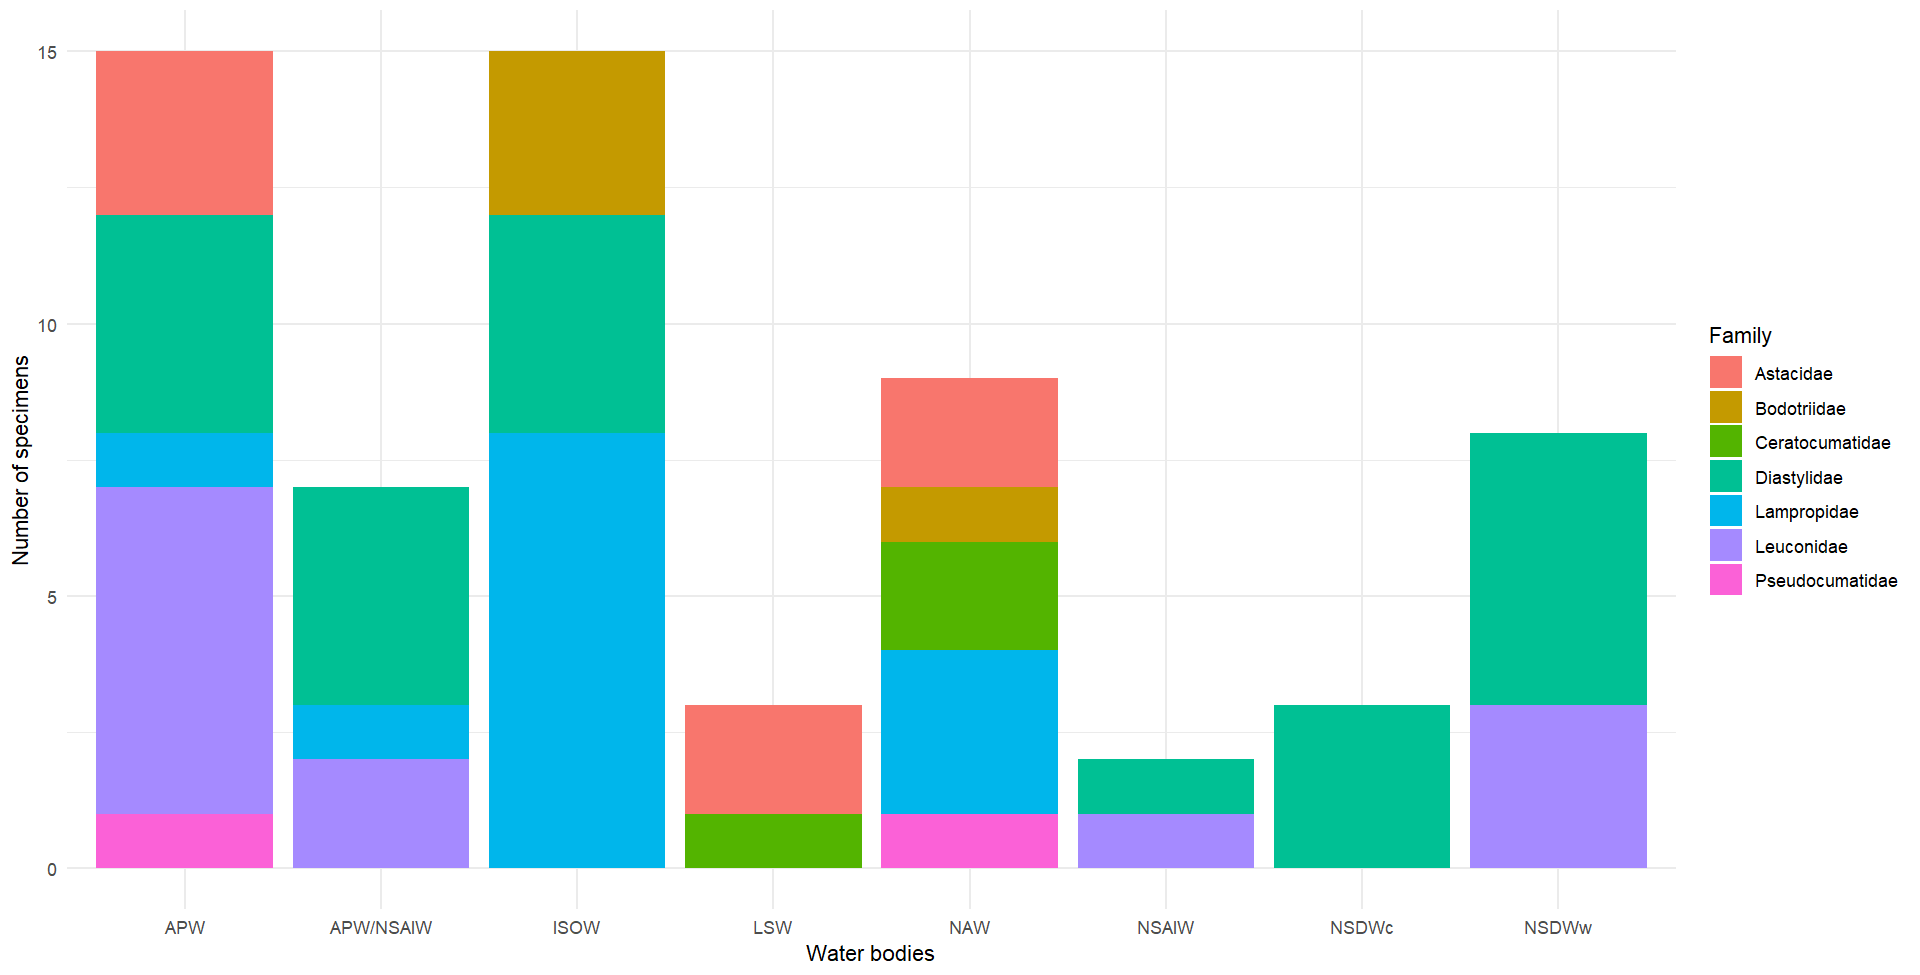
\includegraphics[width=0.7\textwidth]{figure3.png}
    \caption{Histogram of the frequencies of the Cumacea families found in our sample according to the water bodies where they were collected. \label{fig:fig3}}
\end{figure}

Figure \ref{fig:fig3} shows the distribution of samples from different Cumacea families according to the variety of water bodies where they were collected. This makes it possible to compare the diversity and potential preferences of the different families in each body of water. 

APW (Arctic Polar Water) has a high family diversity, with a significant presence of the Leuconidae, Diastylidae and Astacidae. APW/NSAIW (Arctic Polar Water/North Sub-Arctic Intermediate Water) shows a high presence of Diastylidae and Leuconidae, with a low density of Lampropidae. ISOW (Iceland Scotland Overflow Water) has a great abundance of specimens, including Lampropidae and  Diastylidae. LSW (Labrador Sea Water) shows low family diversity, with a preponderance of Astacidae. NAW (North Atlantic Water), like APW (Arctic Polar Water), has a high family diversity, with a predominance of Lampropidae, Ceratocumatidae and Astacidae. NSAIW (North Sub-Arctic Intermediate Water) shows, like LSW (Labrador Sea Water), a low family diversity, represented by the Leuconidae and the Lampropidae. NSWc and NSDWw (North Sub-Atlantic Deep Water, cold and warm), have high abundances of Diastylidae, with the presence of Leuconidae in NSDWw (warm North Sub-Atlantic Deep Water).

\begin{figure}[]
    \centering
    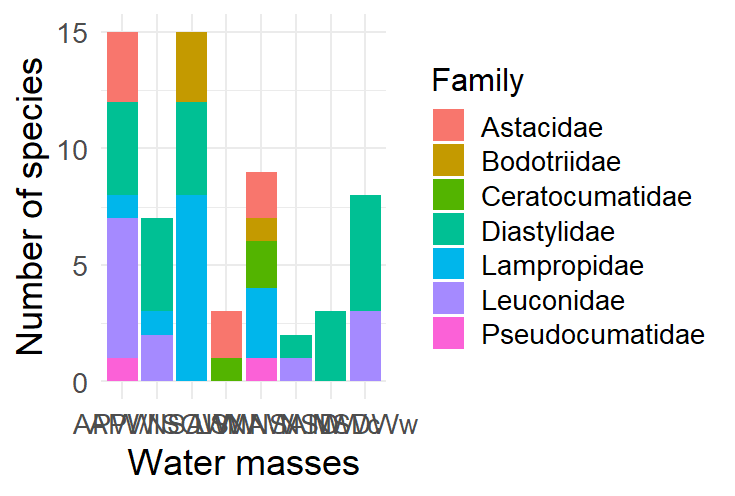
\includegraphics[width=0.7\textwidth]{figure4.png}
    \caption{Histogram of the frequencies of Cumacea families found in our sample according to the habitat where they were collected.\label{fig:fig4}}
\end{figure}

Figure \ref{fig:fig4} shows the distribution of samples from different families of Cumacea according to the type of habitat where they were collected during sampling. This makes it possible to compare the diversity of the different families in each type of housing.

Deep sea, there is a wide variety of families, dominated by the Diastylidae and the Lampropidae. Shelf, presents a wide variety of family, but less than the deep sea. It is dominated by the Leuconidae. Slope, shows low family diversity, with a greater presence of Diastylidae. 

Figures \ref{fig:fig5} and \ref{fig:fig6} below show the degree of correlation between a portion of the multiple sequence alignment (window) of our samples and two climatic parameters: wind speed at the start of sampling (m/s) and the O2 concentration of the water where the samples were collected (mg/L). This correlation was based on 4 metrics: Least-Square Distance, Robinson-Fouls Distance, Normalised Robinson-Foulds Distance and Euclidean Distance. These results were obtained using the functions leastSquare(tree1, tree2), robinsonFoulds(tree1, tree2), euclideanDist(tree1, tree2) from the aPhyloGeo software and were organised by the main function (see \autoref{lst:main}). 

Sequence correlation raises the question of how variations in sequences (windows) respond to or vary with climatic conditions. Conserved positions (low values) could potentially suggest functionally essential regions that do not readily vary with changing climatic conditions, while fluctuating windows (high values) could present specific adaptations to climatic conditions. Analyzing how sequences do or do not vary under these two different climatic conditions can highlight regions in the sequences (windows) that are sensitive or resistant to fluctuations in these two climatic parameters. In our results, we observe a similar fluctuation of the correlation with these two parameters between Figure \ref{fig:fig5} and \ref{fig:fig6}.

\begin{figure}[]
    \centering
    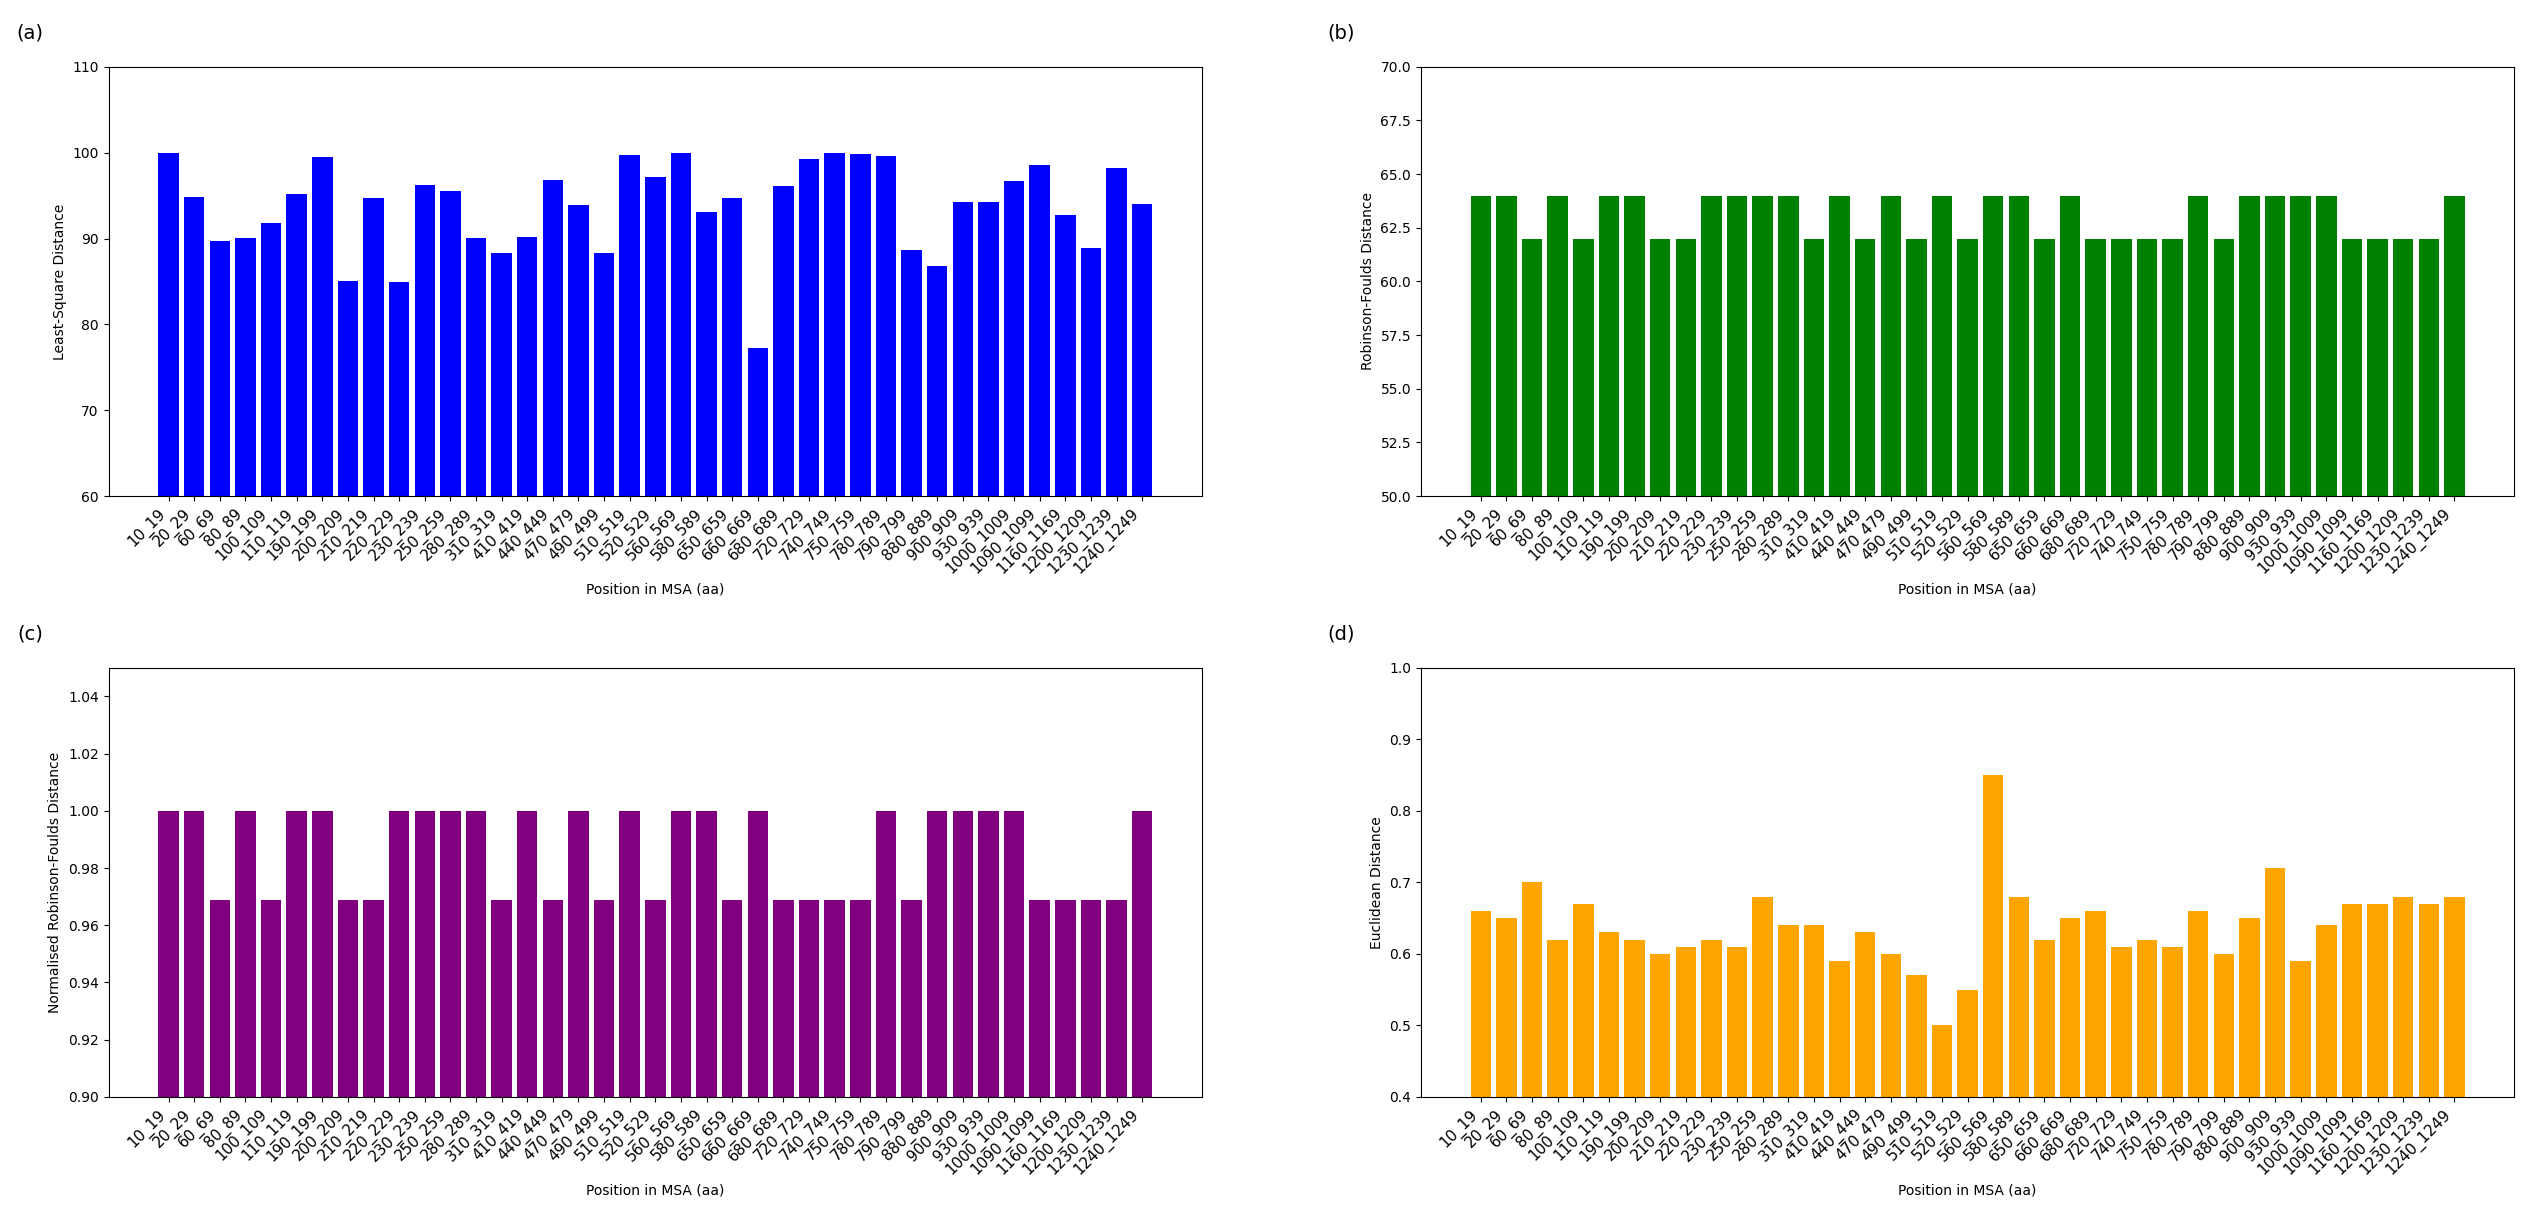
\includegraphics[width=0.7\textwidth]{figure5.png}
    \caption{Variations in the four metrics (Robinson-Foulds distance, generalized Robinson-Foulds, Euclidean distance, and least-square distance) analyzed to elucidate their correlation with fluctuations in wind speed at the start of the sampling (m/s). \label{fig:fig5}}
\end{figure}

In Figure \ref{fig:fig5}a, the peaks and troughs suggest that some locations across the sample sequences are more conserved and therefore similar (smaller distance), probably indicating potential functional or structural significance, while other positions show more variability (larger distance). In contrast to Figure \ref{fig:fig5}a, the values in Figure \ref{fig:fig5}b are more concentrated on restricted values, suggesting a more uniform fluctuation. In this context, lower variation may indicate that changes in sequences do not completely affect local phylogeny. The same is true of Figure \ref{fig:fig5}c, where the normalized distances are rather homogeneous, dictating that variations in sequence positions have a fairly constant impact on the phylogenic structure of the trees. The Euclidean distance, shown in Figure \ref{fig:fig5}d, appears to be the most sensitive and disparate distance to our data. A higher Euclidean distance means a greater difference between sequences at position 520_529 (see Figure \ref{fig:fig5}d), suggesting that this site is more variable or evolutionarily susceptible to change. 

\begin{figure}[]
    \centering
    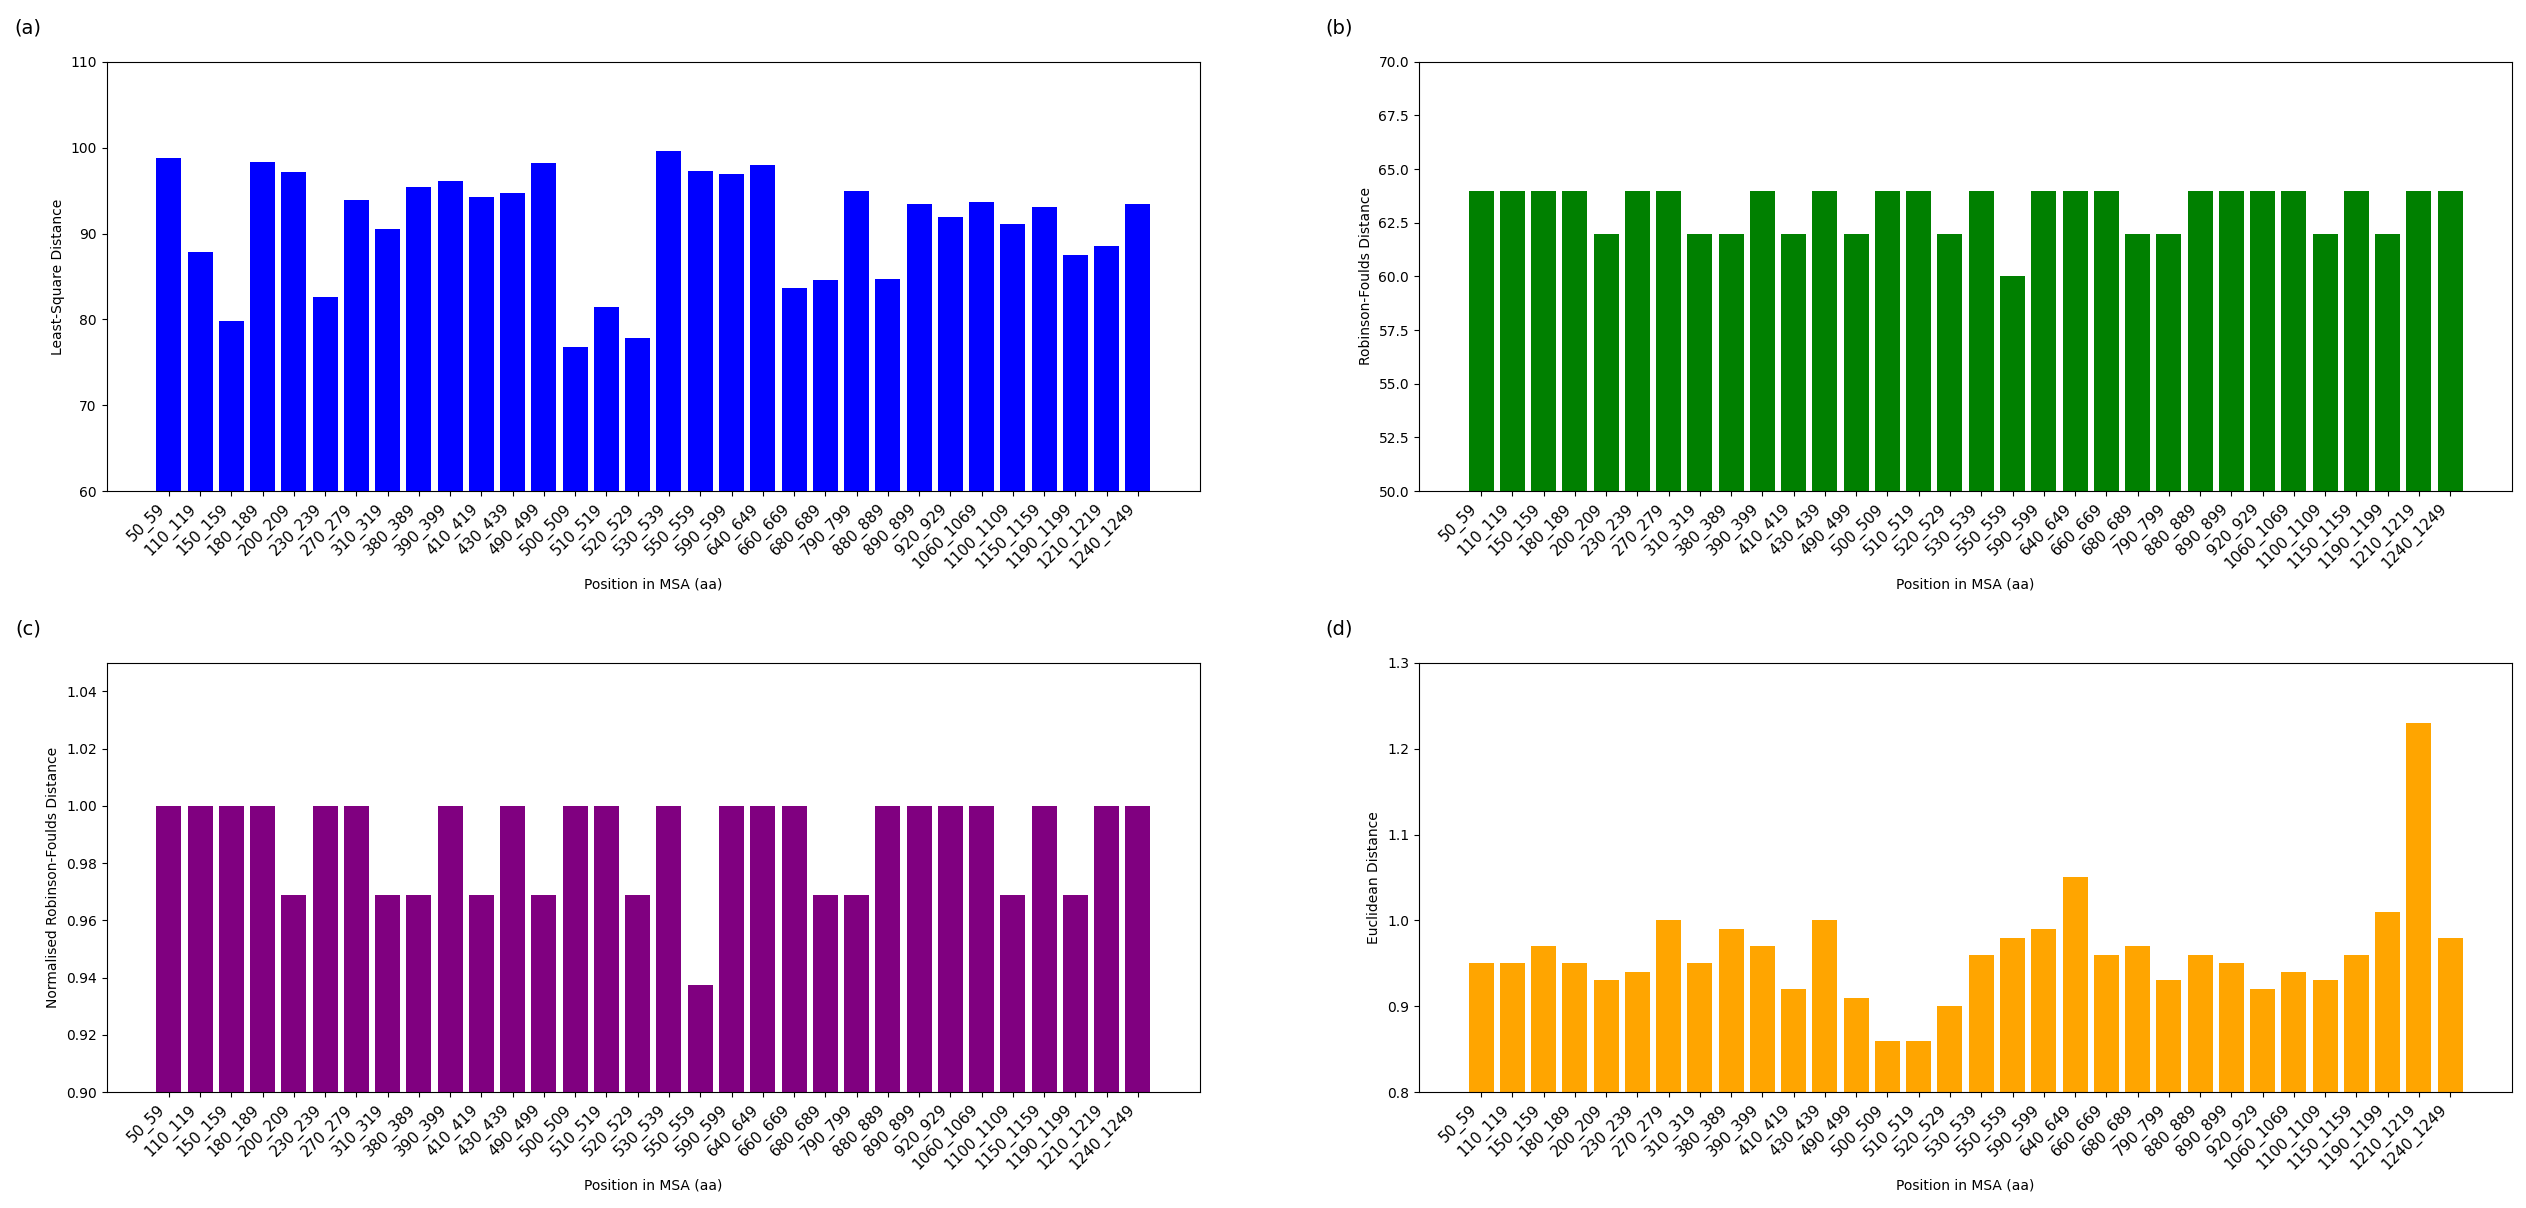
\includegraphics[width=0.7\textwidth]{figure6.png}
    \caption{Variations in the four metrics (Robinson-Foulds distance, generalized Robinson-Foulds, Euclidean distance, and least-square distance) analyzed to elucidate their correlation with fluctuations in O2 saturation ground (mg/L). \label{fig:fig6}}
\end{figure}

Figure \ref{fig:fig6}a is similar to figure \ref{fig:fig5}a, but shows more variation between different window positions. Windows with smaller mean-squared distances are more likely to be evolutionarily conserved, while windows with larger distances show greater instability. The Robinson-Foulds distances in Figure \ref{fig:fig6}b vary with a restricted range of values (50 to 70). These small variations suggest that fluctuations in sequences do not significantly alter local phylogeny. Like the figure above, Figure \ref{fig:fig6}c has a fairly homogeneous distribution. This means that variations in individual window positions exert a fairly uniform influence on the phylogenetic arrangement of trees following normalization. Like Figure \ref{fig:fig5}d, the Euclidean distance presented in Figure \ref{fig:fig6}d shows the greatest sensitivity and heterogeneity from our data. The position with the highest Euclidean distance (1190_1199, see Figure 5d) shows significant dissimilarity between sequences at this position, which may signify a more fluctuating or evolutionarily unstable site. 

All these results will need to be further investigated and analyzed in order to provide a more complete understanding of these results, and thus enable us to draw solid conclusions.

\section{Conclusion}\label{conclusion}

The objective of this study is to perform an in-depth analysis of the influence of extreme climatic variables and environmental characteristics around Iceland on Cumacea (crustaceans: Peracarida) based on phylogeographic analysis. To date, we have selected relevant attributes for our study based on data from the IceAGE project, BOLD Systems, and the study by \citep{uhlir_adding_2021} and eliminated those that were not relevant to this study as well as those that had low variance (salinity, \( S^2 = 0.02146629 \)) or abundant missing data (>95\%). Thus, the first part consisted mainly of literature review, data collection, data pre-processing, and data analysis.
